\documentclass[tikz]{standalone}
\begin{document}
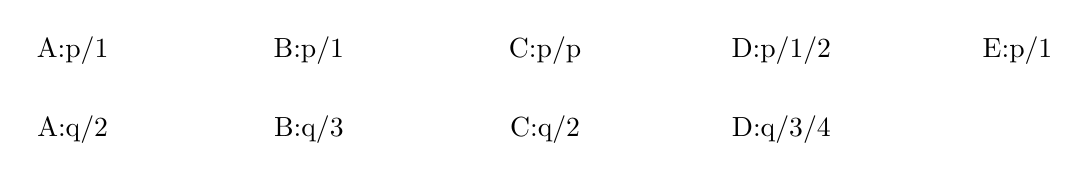
\begin{tikzpicture}[x=1cm,y=1cm]
  \foreach \a/\b [count=\i] in {p/1,q/2} { \node at (0,-\i) {A:\a/\b}; }
  \foreach \a/\b [count=\i] in {p/1/2,q/3} { \node at (3,-\i) {B:\a/\b}; }
  \foreach \a/\b [count=\i] in {p,q/2} { \node at (6,-\i) {C:\a/\b}; }
  \foreach \a/\b/\c [count=\i] in {p/1/2,q/3/4} { \node at (9,-\i) {D:\a/\b/\c}; }
  \foreach \a/\b [count=\i] in {p/1/2/3} { \node at (12,-\i) {E:\a/\b}; }
\end{tikzpicture}
\end{document}
